\documentclass{article}
\usepackage{amsmath}
\usepackage{titling}
\usepackage{float}
\usepackage{graphicx}

\title{Calculus}
\preauthor{}
\author{}
\postauthor{}
\predate{}
\date{}
\postdate{}

\begin{document}

\maketitle

\section{Introduction}
Quite a few people have told me they dislike calculus, or find it a pain. This is, to some extent, understandable. I know very few people who enjoy memorizing formulas, and a common refrain in math is "why not just use [insert calculator of choice here]?" 

Math does have very broad applications, of course, and calculus is no exception - not just in the sciences, but in more humanities oriented subjects as well (though I do admit you will likely not need calculus analyzing literature...then again, you never know!), which are often slightly less recognized. I try to give some examples of these as well.

However, really I think the problem is that when it seems like you're just throwing numbers (or letters, as the case may be) at the wall in an attempt to get them to stick, math seems incredibly frustrating and pointless. Math does have a lot of intuitive reasoning, but it's often not mentioned at all.

There's a few examples of this that can be hit upon quite quickly in algebra. Take finding the area of something, a concept \textit{integral} to calculus (sorry). We're told that for a rectangle it's height times width, and then it's left at that.

But let's actually think about this! Let's pretend we did not go through geometry and try to figure out what the formula for area is - we might be able to guess intuitively it has something to do with length and width, because we know the size of the 2d shape we're thinking about increases as those things increase...but what exactly do we do with length and width?

Well a good first step is to start by defining properties we know the formula for area should have, based off of what we intuitively know for area. For instance, say we have shape one, with a certain length and width. If we place a copy of that shape next to itself - doubling the width - the area overall should double, just from an intuitive sense. So we know that $A(l, 2w) = 2 A(l, w)$. We know this is true if we stack the copies too, and that it's true if we stack three copies, or four, or however many we'd like. So we know that $A(x l, w) = x A(l, w)$ and $A(l, xw) = x A(l,w)$. Alright, we've defined what must be true about area based on some intuitive properties...the next step is generally doing some manipulating.

In this case, what those two rules told us is that we can pull numbers out from inside of the area formula. For instance, $l = 1\cdot l$, and $w = 1\cdot w$...so we can rewrite our formula as $A(l,w) = lwA(1,1)$. What's $A(1,1)$? It's effectively the idea of units. Are we measuring area in light-years? Nanometers? $A(1,1)$ needs to be the area of a single square [unit].

The third bit generally has to do with picking our final equation to make it pretty. We could say $A(1,1) = 13$. There is nothing that stops us from doing this. Area would still follow those intuitive properties we mentioned. \textit{We choose that $A(1,1) = 1$ because it's convenient.} (See the resources section - there's a very good book from which this example is lifted and goes into these ideas in more depth.)

All of the intuition there, the reason why we talk about length times width, and why the equations are the way they are, is not mentioned. And so on, throughout calculus - proofs are mentioned as an aside  if at all (and often when actually mentioned they're gory cramped affairs that explain very little), applications are whole new things to learn instead of consequences of the base ideas, and just in general it feels like a slog.

And here is the point where I'm supposed to say 'but no longer! For just \$19.99 you too can have the shiny Calculus 9000!' This is disingenuous at best. Different explanations work for different people. The lovely thing about calculus, having been around for hundreds of years and being a relatively commonly taught subject, is that there are many, many resources out there, many of which are free (I list some that I've found particularly nice at the end of this). If the explanations here don't make sense to you...try some others! The repetition of the ideas from a new angle will likely assist. 

If you've tried a bunch of different resources and something just desperately does not make sense - ask people who you know are alright at explaining things to try to explain it to you. Find a forum you can ask on, like r/learnmath or math.stackexchange.com. Ask a teacher - if you don't follow your math teacher's explanation, try a science teacher. Try applying the idea to a few problems and see what happens. Talk to a rubber duck (or a stuffed animal, a long-suffering friend, a convenient squirrel, etc) as you work through the problems, explaining what you know and why you are approaching each step the way you are. There is no shame in something taking some time to click.

Quite frequently it is not your fault something doesn't make sense, and the solution is not banging your head against a brick wall. Find a different wall that perhaps has a door.

Finally, calculus is often made harder by the gross algebra or arithmetic in it. (I say this as someone who has many times screwed up a derivative because I forgot, for instance, that 4+2 is not 8.) If you don't remember some of the algebra and trig, go back and look up videos on it, like on Khan Academy or from PatrickJMT, or grab the \textit{For Dummies Algebra Workbook} (the workbook has a bunch of worked through problems, which I found helpful back when I was reviewing algebra). 

\section{Derivatives}
There are two types of calculus - integral calculus, and differential calculus. This subsection will cover differential calculus, which is all centered around derivatives.

\subsection{Definition}
Derivatives are basically a souped-up version of the definition of slope that is used to find the slope at a single point of a curve.

If you start with a line, finding the slope is easy - it's rise over run, or

\begin{equation*}
    m = \frac{y_2-y_1}{x_2-x_1}
\end{equation*}

This should be familiar from Algebra I. The notation here is a little odd though - let's change it to function notation:

\begin{equation*}
    m = \frac{f(x_2) - f(x_1)}{x_2-x_1}
\end{equation*}

Let's also switch from using $f(x)$ to $f(t)$ (because often when using derivatives we're looking at how a function changes with respect to time) and treat the difference between $t_2$ and $t_1$ as $\Delta t$, or the change in $t$ ($\Delta$ as a symbol is almost always used to denote change in a quantity - it is not $\Delta * t$, but one quantity):

\begin{equation*}
    m = \frac{f(t + \Delta t) - f(t)}{\Delta t}
\end{equation*}

(Note here that we've replaced $t_2$ with $t+\Delta t$, and this makes sense because we defined $\Delta t$ as $t_2 - t_1$.) So far, this is just notational changes.

So, let's look at applying the ideas of slope to a curve. If we have two points on a curve, we can find the slope between them:

\begin{figure}[H]
    \centering
    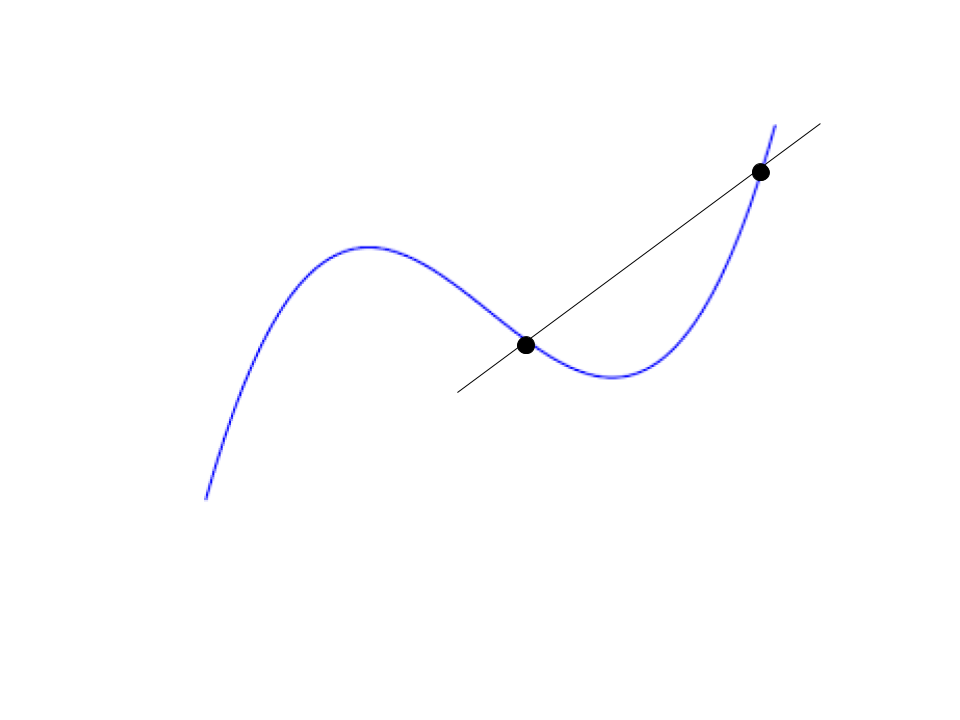
\includegraphics[scale=.15]{diagram1}
\end{figure}

But this isn't very accurate if we're trying to find the slope on, say, the descending limb of this curve. It will get more accurate if we move the two points closer:

\begin{figure}[H]
    \centering
    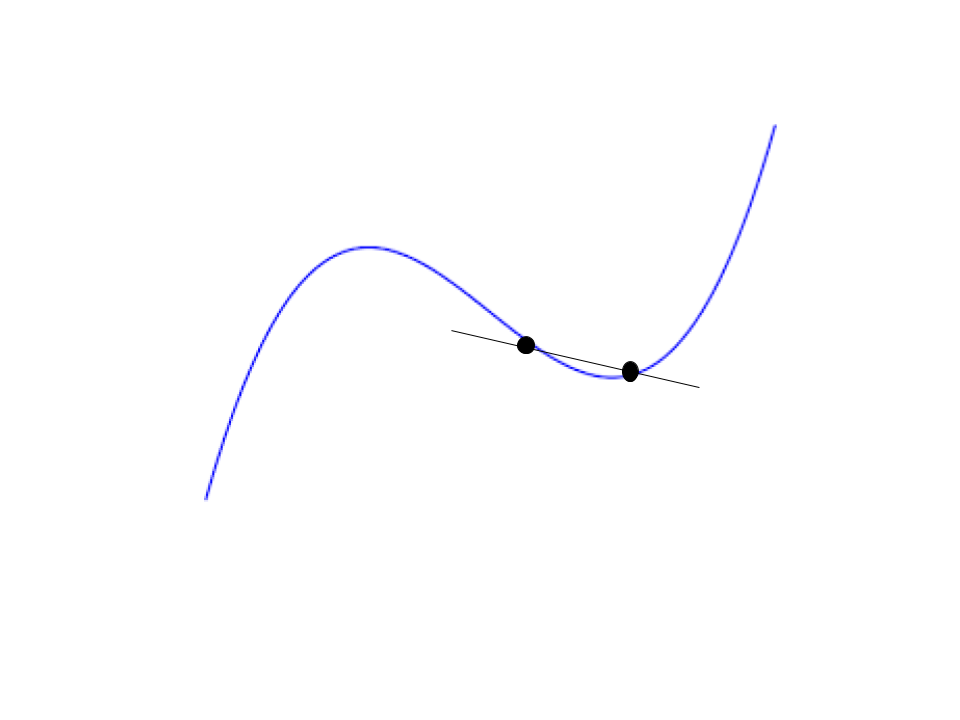
\includegraphics[scale=.15]{diagram2}
\end{figure}

And even closer:

\begin{figure}[H]
    \centering
    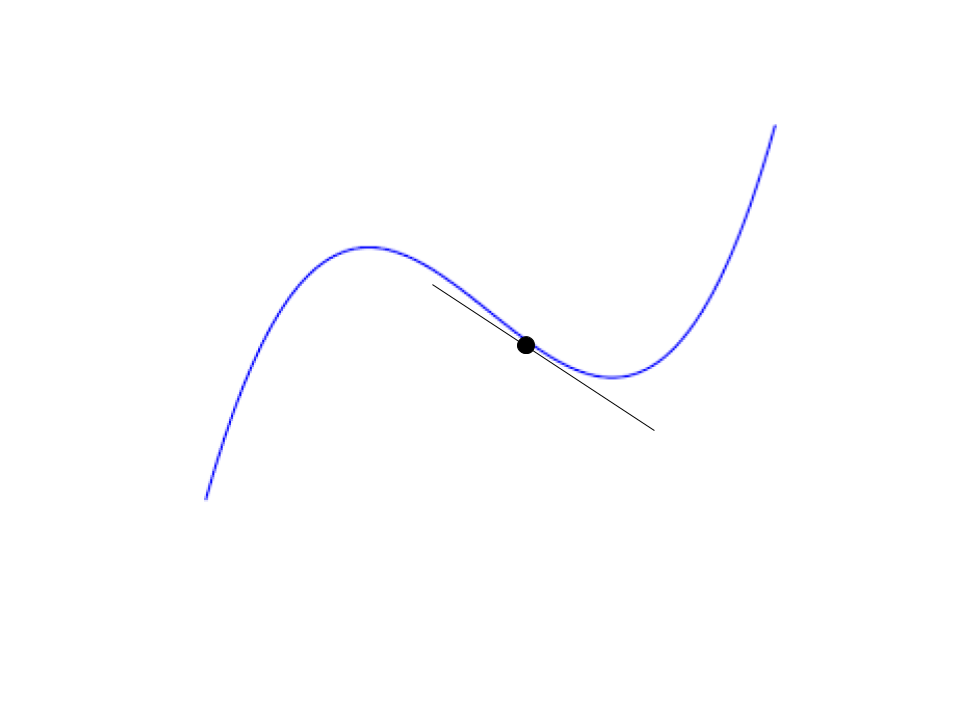
\includegraphics[scale=.15]{diagram3}
\end{figure}

Notice the distance between the points, or $\Delta t$, is approaching zero. (This is called a tangent line - a line that touches a curve at only one point. The earlier lines we drew were secant lines - lines that touch the curve at two points.) So let's add one last piece to our definition of the slope at a single point on the curve:

\begin{equation*}
    m = \lim\limits_{\Delta t\rightarrow 0} \frac{f(t+\Delta t)-f(t)}{\Delta t}
\end{equation*}

What we've added here is something called a {\it limit}. We won't go into the exact definition of a limit just yet, but for now, imagine it as a device that moves those two points closer and closer together for us. You'll probably catch a weird problem here: aren't we dividing by zero?

The answer is a little odd. Basically, we don't let $\Delta t$ approach zero until we've rearranged the equation a bit as we're calculating the derivative. We'll see this in the examples. (A quick side note - $m$ here on out is replaced by $\frac{d}{dt} f(t)$ which is read 'the derivative of $f(t)$ with respect to $t$'. The $d$ is really just a shortcut for $\Delta$, which you'll remember means the change in a particular quantity.)

\subsection{The Power Rule}

Let's do a derivative - say, the function

\begin{equation*}
    f(t) = t^2
\end{equation*}

Begin by plugging this in to our definition of a derivative:

\begin{equation*}
    \frac{d}{dt}f(t) = \lim\limits_{\Delta t\rightarrow 0}\frac{(t+\Delta t)(t+\Delta t) - t^2}{\Delta t}
\end{equation*}

This simplifies to

\begin{equation*}
    \lim\limits_{\Delta t\rightarrow 0}\frac{t^2 + 2t\Delta t + \Delta t^2 - t^2}{\Delta t}
\end{equation*}

or

\begin{equation*}
    \lim\limits_{\Delta t\rightarrow 0}\frac{2t\Delta t + \Delta t^2}{\Delta t}
\end{equation*}

or

\begin{equation*}
    \lim\limits_{\Delta t\rightarrow 0} 2t + \Delta t
\end{equation*}

Here we can now apply the limit, because there's no longer any danger of dividing by zero, and so we get

\begin{equation*}
    \frac{d}{dt}f(t) = 2t
\end{equation*}

Let's sanity check this. Look at a graph of $t^2$ - does the slope look like about $2$ at $x=1$? About $4$ at $x=2$? Remember that that's fundamentally what we're doing - looking at the slope along one section of the curve zoomed in.

That was a lot of work, and it turns out there are several rules that act as shortcuts to doing derivatives. The first of them is a power rule, and it gives the answer to the question

\begin{equation*}
    \frac{d}{dt}t^n
\end{equation*}

where $n$ is any real number. The key point here is looking at what $(t+\Delta t)^n$ looks like. Let's do the multiplication for a few numbers $n$. If $n = 2$:

\begin{equation*}
    (t+\Delta t)^2 = t^2 + 2t\Delta t + \Delta t^2
\end{equation*}

If $n = 3$:

\begin{equation*}
    (t+\Delta t)^3 = t^3 + 3t^2\Delta t + 3t\Delta t^2 + \Delta t^3
\end{equation*}

And you'll notice that if we continue with our definition of the derivative, the first term always gets canceled out by the $-f(t)$ term, and that any term with $\Delta t$ to a power greater than one becomes zero with the application of the limit (the terms with $\Delta t$ are fine because the division by $\Delta t$ cancels that bit out).

So we really know that it's the second term in the sequence that matters, and we know that term is always going to be $nt^{n-1}\Delta t$:

\begin{equation*}
    \frac{d}{dt}t^n = \lim\limits_{\Delta t\rightarrow 0} \frac{t^n + nt^{n-1}\Delta t + ... + \Delta t^n - t^n}{\Delta t}
\end{equation*}

which becomes

\begin{equation*}
    \frac{d}{dt}t^n = \lim\limits_{\Delta t\rightarrow 0} \frac{nt^{n-1}\Delta t}{\Delta t}
\end{equation*}

or

\begin{equation*}
    \frac{d}{dt}t^n = nt^{n-1}
\end{equation*}

which is the power rule for derivatives. (Note: the name for how we worked out $(t+\Delta t)^n$ is the 'binomial theorem'.)

\subsection{Product Rule}

Imagine we have a function like $f(x) = \sin(x)\cos(x)$ or something like that - something that can be rewritten as $f(x) = u(x)g(x)$ (i.e., the product of two functions) - and we want to take the derivative of it. How do we do that? (Try to take a stab at it by finding first the derivative of, e.g, $t^3$, and then the derivatives of, e.g, $t^2$ and $t$. How must they be combined to get them to equal each other?)

Let's plug this in to the formal definition:

\begin{equation*}
    \frac{d}{dt}f(x) = \lim\limits_{\Delta t\rightarrow 0} \frac{u(t+\Delta t)g(t+\Delta t)-u(t)g(t)}{\Delta t}
\end{equation*}

We have to do something that separates $g(t)$ and $u(t)$ out from each other. Maybe we can do something involving factoring - in which case we need to add some terms:

\begin{equation*}
    \frac{d}{dt}f(x) = \lim\limits_{\Delta t\rightarrow 0}\frac{u(t+\Delta t)g(t+\Delta t)-u(t+\Delta t)g(t) + u(t+\Delta t)(g(t)-g(t)u(t)}{\Delta t}
\end{equation*}

The two new terms we've added just add up to zero, but then we can factor:

\begin{equation*}
    \frac{d}{dt}f(x) = \lim\limits_{\Delta t\rightarrow 0}u(t+\Delta t)\frac{g(t+\Delta t)-g(t)}{\Delta t} + g(t)\frac{u(t+\Delta t)-u(t)}{\Delta t}
\end{equation*}

Note that two of these subsections are just the definition of the derivative:

\begin{equation*}
    \frac{d}{dt}f(x) = \lim\limits_{\Delta t\rightarrow 0} u(t+\Delta t)\frac{d}{dt}g(t)+g(t)\frac{d}{dt}u(t)
\end{equation*}

The only thing that's left is applying the limit, which gets rid of the $\Delta t$ in the first term:

\begin{equation*}
    \frac{d}{dt}f(x) = u(t)\frac{d}{dt}g(t)+g(t)\frac{d}{dt}u(t)
\end{equation*}

And this is the product rule.

\subsection{Chain Rule}

The chain rule deals with cases where you want to differentiate a function like $f(x) = (5x)^2$ - that is, functions that can be rewritten as $f(x) = g(u(x))$.

The chain rule is kind of intuitive in some ways - it's a lot like what we do for unit conversions. Imagine we were doing a unit conversion from seconds to minutes of a quantity $c$. Then we might do $c\times\frac{1\text{ minute}}{60\text{ seconds}}$. Similarly, for the chain rule, we're switching 'units' - which thing we're differentiating with respect to:

\begin{equation*}
    \frac{d}{dx}f(x) = \frac{dg}{du}\frac{du}{dx}
\end{equation*}

That is, we're differentiating $g(u)$ with respect to $u$ (in the example above, this would be the derivative of $u^2$) and then multiplying that by the derivative of $u(x)$ with respect to $x$ (in the example above, the derivative of $5x$).

While this may not be a formal proof, the intuition here is quite useful and sufficient for now, but feel free to look up the actual proof or come up with your own.

\subsection{Quotient Rule}

The quotient rule derives fairly cleanly from the product, chain, and power rules. Say we want to take the derivative of a function $f(x) = \frac{g(x)}{u(x)}$. We can rewrite this as $f(x) = g(x)u^{-1}(x)$. Then, we use the product rule:

\begin{equation*}
    g(x)\frac{d}{dx}u^{-1}(x) + u^{-1}(x)\frac{d}{dx}g(x)
\end{equation*}

(Quick note - one can also use an apostrophe to indicate the derivative of something - e.g., $f'(x)$ or $f'$ is the derivative of f. I'll use this occasionally when it'll make something neater.) On the derivative of $u^{-1}$ we can use the chain rule and power rule:

\begin{equation*}
    g(x)(u')(-u^{-2})+u^{-1}g'
\end{equation*}

(Remember $u^{-1}$ is just another way we're writing $u$; since it's in the derivative and we can't simplify it further, we'll leave it be.) Then we can do

\begin{equation*}
    \frac{-gu'}{u^2}+\frac{g'}{u}
\end{equation*}

Finally, we get

\begin{equation*}
    \frac{d}{dx}f(x) = \frac{gf' - fg'}{g^2}
\end{equation*}

And that's the quotient rule!

\subsection{Constants and the addition rule}

These last pieces should be attempted on your own: prove that the derivative of a constant $c$ is always zero, and prove that 

\begin{equation*}
    \frac{d}{dx}\left[u(x) + g(x)\right] = \frac{d}{dx}u(x) + \frac{d}{dx}g(x)
\end{equation*}

Both of these pop right out of the definition of a derivative. (From here, too, one can easily figure out the subtraction rule for derivatives.)

\subsection{When are things not differentiable?}

A function is differentiable if you can find the derivative of it at each point in that function's domain. \textit{This isn't always possible.} Remember our original definition:
\begin{equation*}
    \frac{d}{dx}f(x) = \lim_{\Delta t\rightarrow 0} \frac{f(t+\Delta t) - f(t)}{\Delta t}
\end{equation*}
Sometimes we cannot zoom in properly on a single point (remember we said the limit effectively moves the two points on the secant line closer and closer together until it is a tangent line). For instance, take the following graphs:
\begin{figure}[H]
    \centering
    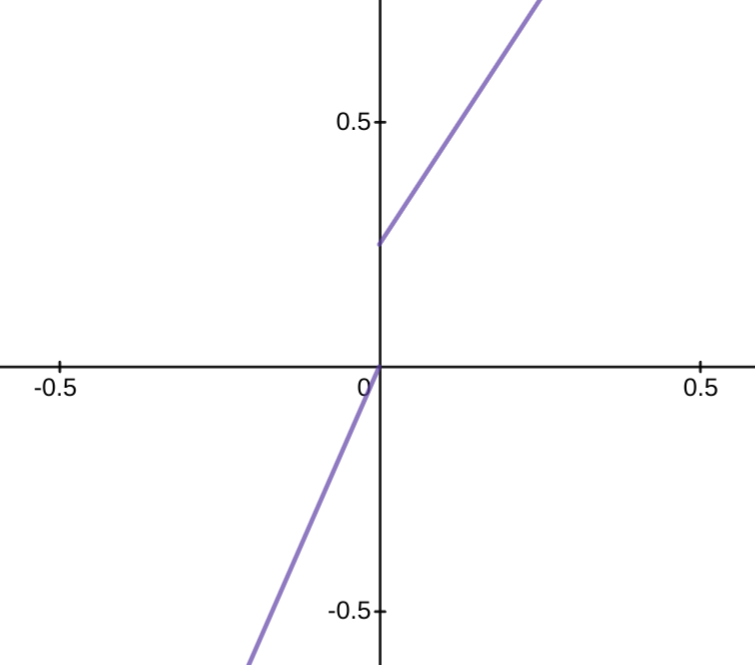
\includegraphics[scale=.1]{split.png}
    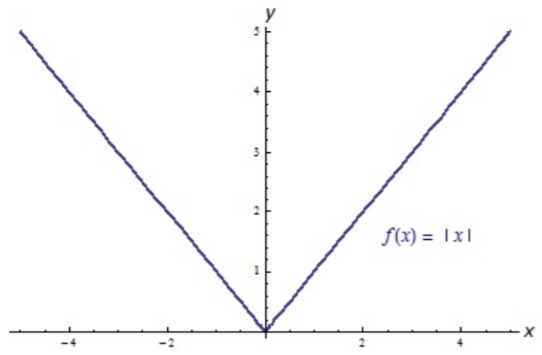
\includegraphics[scale=.15]{corner.png}
    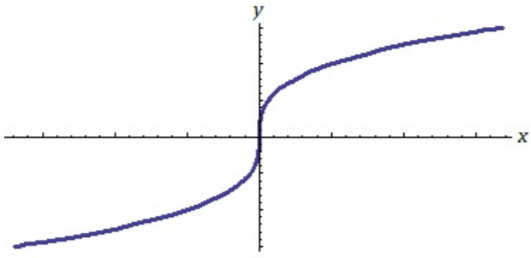
\includegraphics[scale=.2]{steep.png}
    \label{fig:my_label}
\end{figure}

Looking at the first graph, notice that if we tried to take the derivative at zero, we wouldn't be able to have a single tangent line - just looking at the top portion of the graph, it seems like the slope at zero should be 2 or so, but looking at the top portion, it seems like the slope should be 3 or so. There is a disconnect (more formally, the graph isn't continuous) and so we can't find the derivative. (In section 4.3.2, this turns out to be formalized by saying the limits from the left and right aren't equal.)

Looking at the second graph, there's a somewhat similar issue. There's a sharp corner, not a smooth change, which means that as we approach from the left side of the graph, the slope/derivative seems like it should be -1 at zero, whereas from the right side of the graph, it seems like it should be 1. These aren't equal, and we can't find the derivative at that point.

Finally, looking at the third graph, we have a slightly different problem. It's easy to draw a tangent line at zero...but it's vertical. The slope can be best described as infinity, maybe, but it's not something that could be cleaned up if we tried to plug it into our definition of the derivative.

So we can roughly categorize the things we can't take derivatives of as having jumps, corners, or vertical asymptotes.

\section{Applications Part One}
\subsection{Introduction}

A standard calculus textbook has a whole chapter on applications of derivatives, so that's what this is. There's a few examples of why these applications are important and interesting throughout.

\subsection{Extrema, What Graphs Look Like}

The original definition of a derivative has to do with finding the slope of a curve, so let's think about what curves look like.

You'll remember in algebra a lot of time was spent finding intercepts, memorizing the shapes of parent functions, and generally learning how to sketch a graph by hand without Wolfram Alpha. You'll be pleased to note that derivatives make this much easier, and also help us figure out some interesting points that \textit{do} tend to have real life applications: extrema (extremes).

A graph has maximum points and minimum points. Think of a ball on a graph - it'll roll down to minimum points, and maximum points are where it can't get up any higher. You'll also note that some minimum points are lower than others - a ball can roll down to both, but it might end up lower at some minimums than others. This is why we call some maximums and minimums \textit{local} - that is, if we zoom in they seem pretty tall - like how a building in your local neighborhood might be pretty big - but if we zoom out, that building is probably nowhere near as big as the Burj Khalifa, just like the local minimums/maximums aren't as big/small as the overall maximum/minimum.

What's also very interesting at these maximums and minimums is that they have a special property: the slope is zero. To see this, take a minimum: the slope can't be negative; that would mean it's still decreasing and you could reach yet greater depths before your ball rolled to a stop. It couldn't be positive; that would mean your ball is heading out of the minimum. It must be zero - neutral - your ball rolling nowhere.

\textbf{What this means is we can find points where the derivative is zero and those will be our extrema.} Furthermore, we know that spots where there is a positive derivative, the graph has a positive slope, and is therefore increasing in value, and vice versa for negative slope. (If at any point a statement about derivatives confuses you, substitute 'derivative' for 'slope,' graph the statement and see if it makes sense.)

\subsubsection{Let's Calculate This}

Alright, so we know that extrema points have a slope of zero, and we know that if the derivative is positive on an interval, the slope is positive - so we can see from this whether the extrema are maximums or minimums. For instance, let's say we have the function $f(x) = x^2+3x+2$.

First, we take the derivative and set it equal to zero: $f'(x) = 2x + 3 = 0$. If we solve this equation, we get that $x = -\frac{3}{2}$. At this point, we have a potential maximum or minimum point, but we have to check that the graph actually "changes directions" - which we can do by picking a point to the left of $x=-\frac{3}{2}$ and a point to the right and checking if the derivative is positive or negative at each:

\begin{center}
    \begin{tabular}{c|c}
        $x<-\frac{3}{2}$ & $x>-\frac{3}{2}$ \\
         \hline
        E.g., $f'(-2) = -1$, so $-$ & E.g., $f'(0) = 3$, so $+$ 
    \end{tabular}
\end{center}

We can see that there is definitely a 'direction change' in the graph, and furthermore that the graph goes from sloping downward to sloping upward, meaning that this is a minimum - it did not go further down, but turned upward. The ball would stop at the bottom here. We can then find the full point by plugging our $x$ value back into the original function (we're not looking for the slope at that point, but where precisely it's at): $f(-\frac{3}{2}) = -\frac{1}{4}$, so we know the minimum is at $(-\frac{3}{2}, -\frac{1}{4})$. Feel free to graph to double check!

This is the basic principle of this sort of problem, but generally there are more maxima/minima, and the function to take the derivative of is more complex.

\subsubsection{Why We Care}

In many, many situations, extrema are interesting. We often want to optimize for extrema (see the next subsection for details on how to do this) - e.g., the maximum amount of area a fence contains given some amount of fencing material, or the minimum amount of expense given some amount of food needed to be obtained. We're also often interested in the maximums and minimums just for themselves - for instance, in literature (ha. I take back what I said in the introduction) Kurt Vonnegut once said there are six basic story plot arcs. Researchers then plugged a corpus of works into a machine learning model and graphed emotional highs and lows - emotional extrema - to find out if this is true (it is; the paper can be read at https://arxiv.org/pdf/1606.07772.pdf). They were fundamentally interested in how authors manipulate the emotional tone of a text between maximums (joy, happiness) and minimums (sadness, anger) and thereby produce commonalities in plot.

\subsubsection{Optimization Problems}

One specific application, as mentioned earlier, is optimization. For instance, imagine you are an ornithologist studying the cedar waxwing, and you want to know which of several colonies is doing the best. One way to measure how well a colony is doing is how many juveniles survive to adulthood. Of course, it is useful to have a maximum to compare to - with the maximum reasonable density of nests, how close are these colonies getting?

So you, the expert ornithologist, collect data, and find that considering food limitations, carrying capacity, all that jazz, that if $F$ is the number of young fledglings that survive to adulthood per square meter and $D$ is the density of the nests in nests per square meter, the relationship can be approximated by $F = 4D + 2D^2 - 2D^3$. With this equation, you can calculate a maximum for density and fledgling survival to compare your data for each colony to.

This is still just a problem of finding the maximum/minimum, but buried in a lot of words. We know we're trying to find the maximum of $F(D)$, so let's begin by taking the derivative and setting it to zero: $F'(D) = 4 + 4D - 6D^2 = 0$. This is just a quadratic; using a calculator we find that $D = -.55, 1.22$. Looking at this, we can just tell that negative density makes no sense, so we'll take that $1.22$ and plug it into $F(D)$, where we find that $F(1.22) = 4.23$, so a reasonable maximum to compare to as you collect your data for each colony would be $4.23$ birds surviving to adulthood per square meter. (Example stolen and streamlined from Parkhurst's \textit{Intro to Applied Mathematics For Environmental Scientists}.)

\subsection{Concavity: Next Level What Graphs Look Like}
\subsubsection{Second Derivatives, Notation}

It turns out you can take derivatives multiple times. For instance, take the function $f(x) = x^3 + x^2 + x + 1$ - $f'(x) = 3x^2 + 2x + 1$ as per the power and addition rules, but we can do this again, treating $f'(x)$ like we would any other function, getting $f''(x) = 6x + 2$ - and again, to get $f'''(x) = 6$, and again to get $f''''(x) = 0$...and again, and again, and again as many times as we'd like. Successive derivatives can be noted by adding an extra apostrophe or by writing $\frac{d^n x}{dx^n}$. There is also the particular case of physics where derivatives are taken with respect to time a lot, and in which case dots on top of the function are used - e.g. $\dot x, \ddot x, \dddot x$, etc.

\subsubsection{Concavity and Points of Inflection}

If first derivatives can be intuitively understood as slope, second derivatives can be intuitively understood as the slope of the slope. In other words, the second derivative asks whether the graph is getting steeper or shallower - how steep are the walls the ball is rolling up or down? Is rolling it uphill practically throwing the ball straight up?

This idea is called concavity, and there are two types: concave up (like a bowl) and concave down (like a hat). These just distinguish the sign of the concavity - does an increase in steepness mean the ball is plummeting into an abyss at an even faster rate, or that it is shooting to new heights?

Calculating where the direction of concavity changes means finding out where the steepness is zero, or in other words, finding out where the second derivative is zero. In this case we use the same approach as we did with maxima and minima, except these points where direction of concavity changes are called points of inflection.

\subsubsection{Why We Care}

Much like maxima and minima, points of inflection have many applications. In finance, for instance, points of inflection could indicate the impending rapid growth of a company's stock or the possible burst of a bubble. 

\subsection{Theorems That Really Shouldn't Have A Name}

\subsubsection{Rolle's Theorem}

If you have a differentiable function and a closed interval where the endpoints have equal $y$ values (are at the same height) the derivative, or slope, must be zero at some point between those two endpoints. If it's a straight line, the slope of the whole thing will be zero. If it curves at all, there will be maxima and minima with a slope of zero at that point. 

I try to remember the name by thinking about a piece of bread (preferably a roll) rolling between either end point, but I always end up forgetting it. If you have a good way to remember the name, please let me know.

\subsubsection{Mean Value Theorem}

A wrong clock is right twice a day, or so the saying goes. In much the same way, the Mean Value Theorem says that given you have a function that is differentiable on a closed interval, there must be a point on that interval where the derivative is equal to the average slope over the interval.

Think of a car on a long road trip. We can get the average speed by looking at the start speed, end speed, and time the whole trip takes, but this won't account for slowing down because of traffic, speeding up because it's late at night and there are no cops around, coffee breaks, \&c. We can look at the derivative at a bunch of these points to find the speed at them. But along that trip, there has to be some point where the average speed equals the speed at that current moment. 

This makes sense, because we know the average is the 'middle' speed - there are points where we might speed up and slow down, but most of the time we're at that middle speed, or passing through it (remember speed is a continuous value - that's why it needs to be a differentiable function). 

\subsubsection{Why We Care}

Rolle's Theorem is used to prove the Mean Value Theorem. The Mean Value Theorem will strike again later (see section 4.3.3 and section 5).

\subsection{Equation of a Tangent Line}

Say you not only want to find the slope of a curve at a point, but in fact the equation of the tangent line at that point.

For example, if we want to find the equation of the tangent line to $f(x) = 2x^2$ at the point $(2, 3)$. First, we know that the equation of a line can be written as $y - y_1 = m(x - x_1)$, so let's find $m$, the slope - in other words, $f'(x) = 4x$. But we want to know the slope, in particular, at $(2,3)$ or where $x = 2$ - so plug this in, and we find $f'(2) = 4(2) = 8$. So we know $y - y_1 = 8(x-x_1)$ - and we're given $(x_1, y_1) = (2,3)$, so we can just plug that in to get $y-3 = 8(x-2)$. We're done. We could simplify, but often we don't have to.

\subsubsection{Why We Care}

Tangent lines can help us approximate points for a particularly complicated function by using a bunch of short tangent lines to approximate the curve. This is used, for instance, in Newton's Method and Euler's Method (ways of finding roots and solving differential equations, respectively - the latter is briefly covered in section 8), both of which have their own far ranging applications.

\subsection{Implicit Differentiation}

Implicit differentiation is a good way of getting around a common problem - finding the derivative when you can't easily solve for $y$ or $f(x)$. The basic idea is this: say you have a function like $1 = x^2 + y^2$. Sure, you could technically solve for $y$, but that'd be nasty. The other option is using the chain rule. Let's differentiate each side with respect to $x$:
\begin{align*}
    \frac{dy}{dx} 1 &= \frac{dy}{dx}x^2 + y^2\\
    0 & = 2x + \frac{dy}{dx} y^2
\end{align*}

From here, treat $y$ as some complicated function, and do the chain rule:

\begin{equation*}
    0 = 2x + 2yy'
\end{equation*}

We just multiplied by the derivative of $y$, but since we don't know what $y$ is, we called it $y'$...which is awfully convenient, because that's what we're looking for. Now we just solve for $y'$:

\begin{equation*}
    y' = \frac{dy}{dx} = -\frac{2x}{2y} = -\frac{x}{y}
\end{equation*}

That's all implicit differentiation is - abusing the chain rule so we can take the derivative without solving a nasty equation.
\subsubsection{Why We Care}

There's an interesting little consequence of implicit differentiation - it makes it really easy to find the derivative of functions that are inverses of each other when you only know the equation of one of the functions.

We'll make use of this detail when talking about derivatives of inverse trig functions in section 5.3.

\subsubsection{Related Rates}

Another use of implicit differentiation is in 'related rates' problems. The easiest way to see how they work is just to do an example: say you have a spherical balloon being filled at a rate of 4.5 cubic feet per minute. The problem might ask you to find the rate of change of the radius when the radius is 2 feet. 

The key with these problems is simply carefully spelling out variables, and finding out the equation that will allow you to take it from two variables to one variable.

Note that I will be using shorthand here, but if it makes it easier for you when solving these, feel free to spell out $d[\text{balloon volume}]$ instead of just $V$, for instance. Often doing this makes it easier to keep track of what precisely is going on.

So we know the rate of increase of volume, or $\frac{dV}{dt}$, is $4.5 \text{ ft}^3\text{/min}$. We also know that the balloon is spherical, so the volume can be described by the equation $V = \frac{4}{3}\pi r^3$. We're looking for the rate of the change of the radius, so $\frac{dr}{dt}$ when $r=2$.

First, let's take the derivative of the equation for the volume of a sphere with respect to time, $t$:
\begin{align*}
    V &= \frac{4}{3}\pi r^3\\
    \frac{dV}{dt} & = \frac{dV}{dt}\frac{4}{3}\pi r^3\\
\end{align*}

Here's where implicit differentiation comes in:
\begin{equation*}
    \frac{dV}{dt} = \frac{4}{3}\pi 3r^2\frac{dr}{dt}
\end{equation*}
Now, we are trying to find $\frac{dr}{dt}$, so let's solve for that (I'm substituting $V'$ and $r'$ in for $\frac{dV}{dt}$ and $\frac{dr}{dt}$):
\begin{equation*}
    \frac{3V'}{4\pi 3r^2} = r'
\end{equation*}

We are given $V' = 4.5$ and that at the moment we are interested in, $r = 2$ (note that sometimes you have to watch the units here, but in this case everything is in feet and minutes so we don't have to worry), so we can just plug those in:
\begin{equation*}
    r' = \frac{3(4.5)}{4\pi 3(2)^2} = \frac{9}{32\pi} \approx 0.09 \text{ ft/min}
\end{equation*}

\section{Interlude: Limits}
\chapter{Intuition of Limits}
The purpose of limits is to find what a function approaches at a certain number that it is not defined for. 
For example, let's say we have the function $f(x) = \frac{x^2}{x}$ and $x = 0$ in this particular case. 
Since we are not allowed to divide by zero, this function is not defined there. 
However, the function may approach a certain number.

\begin{figure}[H]
\caption{Function approaching $1$ as $x$ goes to $0$}
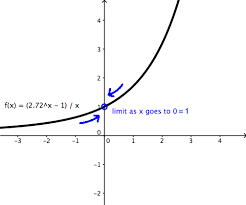
\includegraphics[scale=0.8]{../images.png}
\end{figure}

In the above graph, while the function is not defined at $0$, it approaches, or comes near to, $1$. 
There are several different "types" of limits and rules for calculating them. 
\chapter{Types of Limits}

The first type of limit you could call an "easy" limit. 
All you have to do is plug in the number you are approaching for your variable, because the function doesn't violate any rules like we described above. 
So for example, if you have the limit

\begin{equation*}
    \lim\limits_{x\rightarrow 1} x
\end{equation*}

You would just get 1. 
The second type of limit could be called a "$\frac{0}{0}$" limit. 
It does violate the rules, and we have to do some algebraic manipulation to get it into a form we can work with. 
This might be done via factoring a polynomial, normalizing the denominator or numerator, or some such method.

A quick algebra side-note here on how to do these things. 
Factoring a polynomial mainly references factoring quadratics, or equations of the form $ax^2 + bx + c$ ($=0$). 
We factor the left side by using this general method: find the factors of $ac$ and see which add up to $b$. 
Note that you can change the signs of the factors, that is, if you have $ac = 10$ and the factors are $1, \, 2, \, 5, \, 10$, and $b = 3$, you can do $5-2 = 3$. 
After this, we then take those two numbers, $5$ and $-2$ and rewrite it as $ax^2 + 5x -2x + c$. 
We then put parentheses in: $(ax^2 + 5x) + (-2x + c)$. 
Finally, we factor out the biggest common number (or variable) out of each of the parentheses.

Let's do this with a real problem. 
\begin{equation*}
    x^2 - x - 12
\end{equation*}
For $ac$, we get $1\times -12$, or $-12$. 
For $b$, we get $-1$. 
The factors of $12$ are $1, \, 2, \, 3, \, 4, \, 6, \, 12$. $-4\times 3 = -12$ and $-4+3 = -1$. 
So now we write 
\begin{equation*}
    x^2 - 4x + 3x - 12
\end{equation*}
Now, we put in the parentheses and get
\begin{equation*}
    (x^2-4x)+(3x-12)
\end{equation*}
Now for the last step, factoring. 
For the first parenthesis, we can take out $x$, and in the second parenthesis, we can take out $3$, so we get
\begin{equation*}
    x(x-4)+3(x-4)
\end{equation*}
Note that if the two parenthesis' contents are not the same, then you have done something wrong. 
Now, we can rewrite this expression as 
\begin{equation*}
    (x+3)(x-4)
\end{equation*}
The equation is now factored.

The other thing of note here is rationalizing the denominator or numerator. 
Normally, we rationalize the denominator to get a radical out of the denominator, but we can also do this for the numerator. 
To do this, we multiply by expression on the numerator or the denominator over itself. 
Let's say we have the expression $\frac{\sqrt{x}}{1}$. 
Then we would multiply by $\frac{\sqrt{x}}{\sqrt{x}}$ and simplify. 
Note that if instead we had an expression like $\frac{\sqrt{x}+1}{1}$ we would multiply by $\frac{\sqrt{x}-1}{\sqrt{x}-1}$. 
We switched the sign on the $1$ from $+$ to $-$. This is called taking the "conjugate" of the expression.

With these tools in hand, we can now start solving the second type of limit. 
Let us take as an example 
\begin{equation*}
    \lim\limits_{x\rightarrow -3}\frac{x^2-x-12}{x+3}
\end{equation*}
We can clearly see that if we just plug it in, there will be a zero in the denominator. 
Instead, we can try employing an algebraic tool. 
You might recognize the quadratic on the top as the one we factored earlier. 
Let us then replace that expression with its factored form:
\begin{equation*}
    \lim\limits_{x\rightarrow -3}\frac{(x+3)(x-4)}{x+3}
\end{equation*}
Now, we can cancel the $x+3$ on the top and bottom of the fraction. 
This then leaves us with
\begin{equation*}
    \lim\limits_{x\rightarrow -3}x-4
\end{equation*}
The limit is now one of our "easy" limits, so we can simply plug in $-3$. The answer is $-7$.

Now we have our final type of limit, the "$\frac{\text{not zero}}{0}$" limit. 
This type of limit is a bit different from the other two types of limits. 
It requires a bit more intuition. As an example, let's say we are trying to solve the problem
\begin{equation*}
    \lim\limits_{x\rightarrow 0}\frac{1}{x}
\end{equation*}
To solve this, we must first solve
\begin{equation*}
    \lim\limits_{x\rightarrow 0^+}\frac{1}{x}
\end{equation*}
and
\begin{equation*}
    \lim\limits_{x\rightarrow 0^-}\frac{1}{x}
\end{equation*}
First, let's examine the second problem. 
The $+$ sign means it is a right limit - that is, we are approaching zero from the left. 
What does that mean? Well, let's say we have a number line like the one below.

\begin{figure}[H]
\caption{Approaching zero}
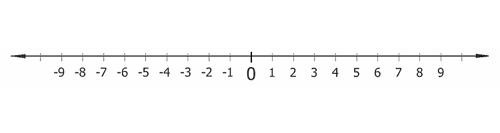
\includegraphics[scale=0.75]{../numberline.jpg}
\end{figure}

To approach from the right means that $x$ will be represented by tiny positive numbers, like $0.00001$ and $0.0000001$. 
They will get closer and closer to $0$. 
So, what does this mean? 
It means the answer to this particular limit will be whatever $\frac{1}{\text{really small positive number}}$ is. 
So let's take some examples. 
If we have $\frac{1}{0.00001}$ we get $100000$. 
If we have something closer to zero, like $\frac{1}{0.0000001}$ we get $10000000$. 
In other words, we are approaching infinity.
So the answer to this limit, approached from the right, is $+\infty$, or just $\infty$. 
Now, let's do the next one. 
This time, we are approaching zero from the left. Now we are dividing by small negative numbers. Try a few on a calculator and see what you get!

It turns out that this approaches $-\infty$. 
So the answer to the third limit in that list we started with is $-\infty$. 
Now, to solve the first limit. 
If we take the second two limits and their answer is the same, the first limit has a solution: the answer to the second two limits! 
However, the second two limits had different solutions. That means the answer to the first limit is undefined.


\section{Derivatives Strike Back}
Or: dealing with trig functions, exponential functions, and logarithms. I'll try to quickly recap relevant rules from algebra as they come up, but again, if this stuff is rusty, try looking at Khan Academy, PatrickJMT, or another similar resource.

\subsection{Normal Trig}

\subsection{Inverse Trig}

Remember that by using implicit differentiation we can find the derivative of inverse functions - and now we know about the derivatives of standard trig functions, so we can now find the derivatives of inverse trig functions (just what we all wanted).

\subsection{Exponentials and Logarithms}

\begin{equation*}
    \frac{d}{dx}\ln x = \frac{1}{x}
\end{equation*}

(We can actually prove the above from the derivative of $e^x$ - see if you can do it!)

\begin{equation*}
    \frac{d}{dx}\log_a x = \frac{1}{x \ln a}
\end{equation*}

The above can be proved from the derivative of $\ln x$ and the change of base formula for logarithms - again, try to do it!

\section{Integrals}
use area of circle proof as example
\subsection{Definition}
\subsubsection{Definite vs. Indefinite}
\subsection{It's All Coming Together}
\subsection{Solving}
Integrals are harder than derivatives. Half of solving them isn't knowing how integrals work, it's manipulating what's beside the integral sign so you can actually do something with it - and even then it's not always possible to find an equation for the solution. Numerical integration is a whole field for a reason. Most people look for a simple trick or two and then use a calculator like Wolfram Alpha to help them out, but it is useful to know some of the standard tricks out there for approaching problems.
\subsubsection{Numerically}
\subsubsection{Subsitution}
\subsubsection{Integration by Parts}
\subsubsection{Trigonometric Substitution}
\subsubsection{Partial Fractions}
\subsubsection{Tabular Method}
\subsubsection{Improper Integrals}

\section{Applications Part Two}
A standard calculus textbook has a whole chapter on applications of integrals, so that's what this is. There's a few examples of why these applications are important and interesting throughout. Note that differential equations are broken out into a separate section.

\subsection{Area Between Two Curves}

\subsubsection{Why We Care}

\subsection{Stuff With Solids}

\subsubsection{Volume}

\subsubsection{Arc Length and Surface Area}

\subsubsection{Why We Care}

\subsection{Some Other Common Applications}

This lists common applications that come up in classes but in reality applications for integrals are everywhere. It should be fairly obvious that they're in the hard sciences, but they also show up in economics (), social science (), and even humanities oriented subjects like \_ or \_. It makes sense why the physics applications are the ones always mentioned as they're the obvious, but it'd do everyone a service if the others were mentioned more.

\subsubsection{Work}

\section{Differential Equations}
\input{difeqs.tex}

\section{Sequences and Series}

\section{Resources}
Some common single-variable calculus textbooks out there are Larson and Edwards' (more high school oriented) and Spivak's (more college oriented, but I've heard it's very good - unlike Apostol's, which I have read some of and detest with a passion as it's thorough but incredibly dry). Like any book on this list, if you can't find a cheap copy at a used bookstore or a free one through a library, you definitely shouldn't try pirating it through LibGen (gen.lib.rus.ec). Definitely not. Ahem.
\begin{itemize}
    \item Paul's Online Math Notes (I don't think they're great for learning, but they are good for reference and have problems with solutions along with proofs of everything.)
    \item Project Gutenberg has several free calculus books online, including Silvanus Thompson's {\it Calculus Made Easy}, which is very good.
    \item I don't much like Khan Academy's videos personally, but they have a ton of practice problems, and can give you an idea of how much of the whole subject you've mastered.
    \item While I haven't personally read it (it's on my list), I've heard very good things about Tarasov's Calculus - it's also free as a pdf online.
    \item If you get stuck, need help with a problem, or similar, try Math Stack Exchange (some of the questions are also just interesting reading in their own right).
    \item 3blue1brown on YouTube has an excellent series on  how calculus works, with beautiful graphics.
    \item \textit{Burn Math Class} - wonderful explanations of many different parts of math, including calculus, along with satisfying tirades about the tragedy that is the American educational system. Where the example with area in the introduction is from. Frankly, would highly recommend you read this above quite possibly anything else on this list.
\end{itemize}
\end{document}
